\documentclass[12pt]{article}

\usepackage[margin=1in]{geometry}
\usepackage{setspace}
\usepackage{enumitem}
\usepackage{titlesec}
\usepackage{graphicx}
\usepackage{hyperref}
\usepackage{amsmath}

\setstretch{1.1}
\setlength{\parskip}{0.5em}
\setlength{\parindent}{0pt}

\begin{document}

\begin{center}
    {\Large \textbf{Patient-Similarity Graph Convolutional Network for Lung Nodule Malignancy Classification on CT Scans}}\\[1.5em]

    Swathi Gopal\\
    Harrison Lavins\\
    Rensildi Kalanxhi\\[1em]

    CSC 7760 Deep Learning\\
    Professor Ming Dong\\
    April 6, 2026
\end{center}

\section*{Goal}

The primary goal of this project is to determine whether modeling inter-nodule similarity as a graph improves lung nodule malignancy classification compared to classifying each nodule independently. Specifically, we construct a patient-similarity graph in which each node represents a lung nodule characterized by CNN-extracted imaging features, and edges connect nodules with similar visual characteristics. A Graph Convolutional Network (GCN) then classifies each node as benign or malignant by aggregating information from neighboring nodes in the graph. We compare this graph-based approach against a standard multilayer perceptron (MLP) baseline that uses identical features but ignores inter-nodule relationships. A secondary goal is to evaluate whether the GCN's graph-based label propagation provides an advantage in low-label (semi-supervised) settings, where only a fraction of nodules have known malignancy labels.

\section*{Background}

This project lies at the intersection of \textbf{medical research} (lung cancer diagnosis) and \textbf{computer vision} (CT image analysis), applying \textbf{graph-based deep learning} to a clinical classification task.

Lung cancer is the leading cause of cancer-related mortality worldwide, and early detection of malignant pulmonary nodules from CT scans is critical for patient outcomes. Deep learning approaches, particularly convolutional neural networks (CNNs), have achieved strong results in nodule malignancy classification on the LIDC-IDRI benchmark (AUC 0.88--0.96). However, these methods classify each nodule independently, ignoring potentially useful relationships between nodules.

Graph Neural Networks (GNNs) offer a complementary paradigm: by representing data as a graph and performing message passing between connected nodes, GNNs can leverage structural relationships that CNNs cannot capture. In cancer research, patient-similarity graphs --- where nodes are patients and edges connect those with similar clinical or imaging profiles --- have shown improved classification for cancer subtyping (ERGCN, Frontiers in Genetics 2022), prognosis prediction (MMGCN, Computers in Biology and Medicine 2024), and multi-omics integration (MOGONET, Nature Communications 2021). However, this patient-similarity GNN paradigm has not been applied to lung nodule malignancy classification on CT imaging data.

Our project fills this gap by applying a standard GCN (Kipf \& Welling, ICLR 2017) to a k-nearest-neighbor similarity graph constructed from frozen ResNet18 features of LIDC-IDRI nodules. The approach is motivated by the clinical intuition that ambiguous nodules near the benign-malignant decision boundary may be better classified when their similarity to confidently labeled nodules is explicitly modeled.

\section*{Deep Learning Model}

The project uses a two-stage architecture, illustrated in Figure~\ref{fig:architecture}.

\begin{figure}[h]
    \centering
    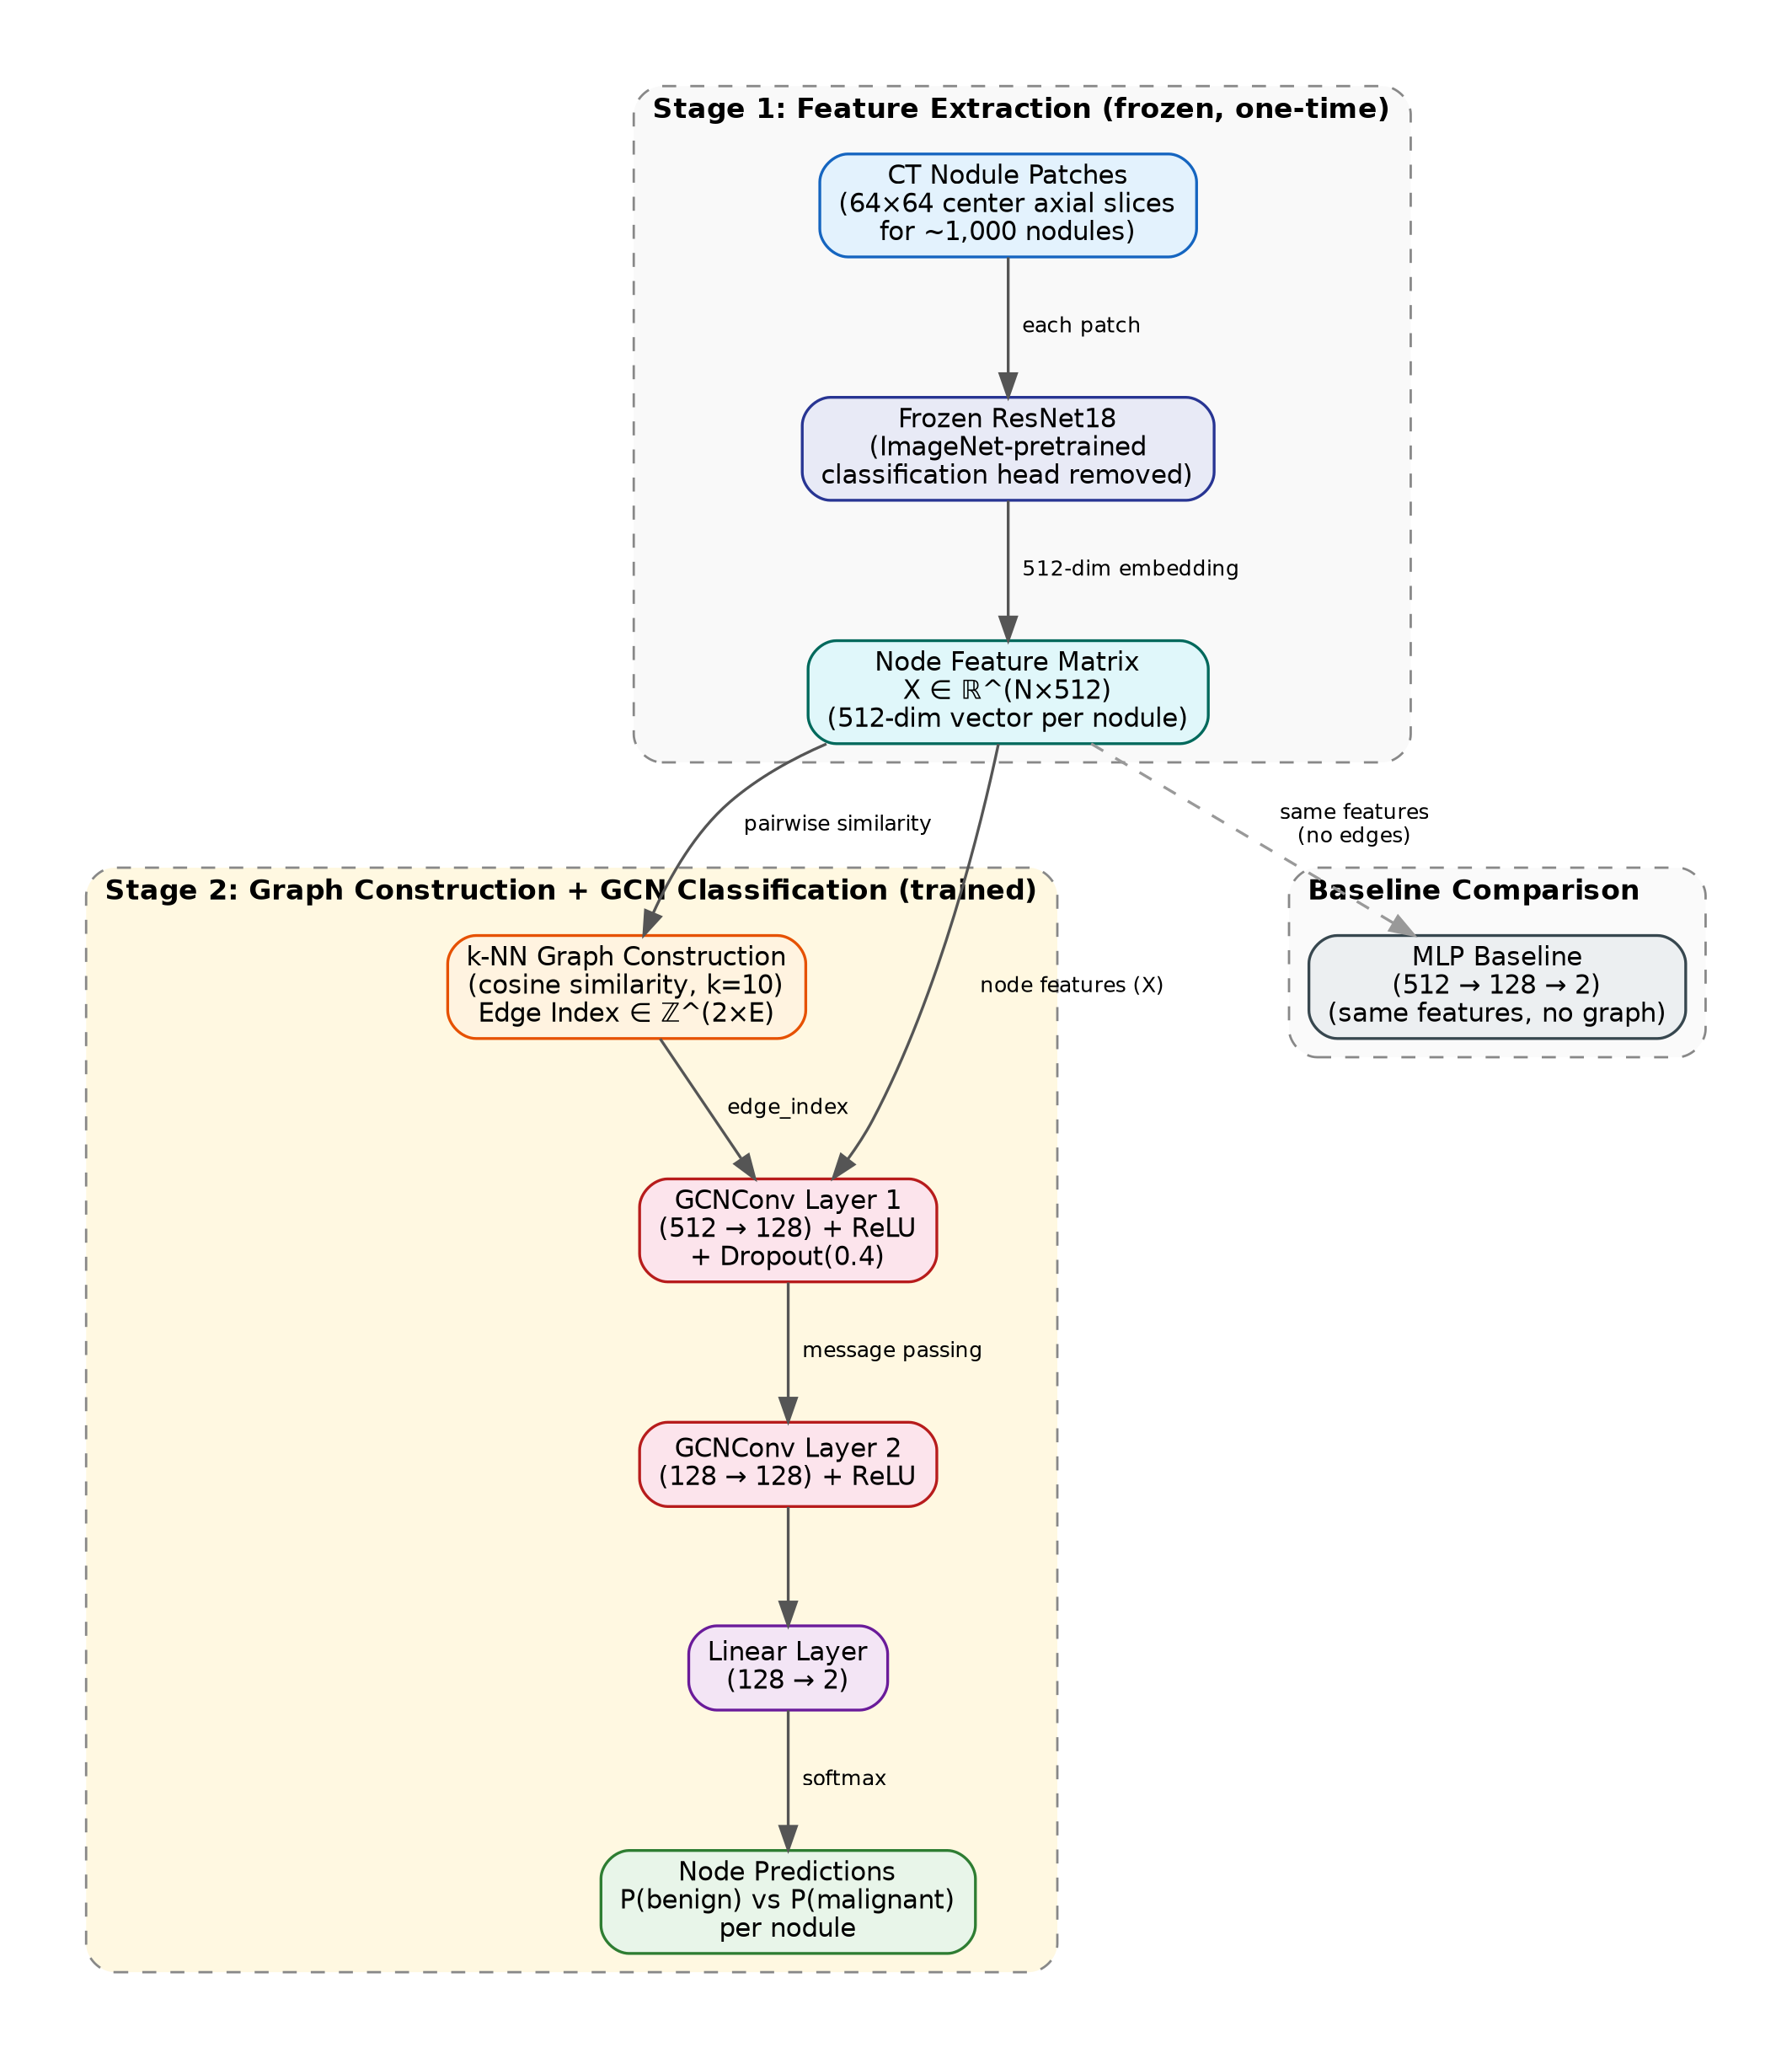
\includegraphics[width=0.75\textwidth]{../../architecture_diagram.png}
    \caption{Two-stage pipeline. Stage 1 (top) extracts 512-dim feature vectors from CT nodule patches using a frozen ResNet18. Stage 2 (left) constructs a k-NN similarity graph and classifies nodes with a 2-layer GCN. The MLP baseline (right) uses the same features without graph structure.}
    \label{fig:architecture}
\end{figure}

In Stage 1, an ImageNet-pretrained \textbf{ResNet18} (frozen, no fine-tuning) serves as a feature extractor: each nodule's center axial slice (64$\times$64 pixels, resized to 224$\times$224) is passed through the network to produce a 512-dimensional feature vector. This step runs once for all nodules and takes approximately 10 minutes on an RTX 3060.

In Stage 2, a \textbf{2-layer Graph Convolutional Network (GCN)} with 128 hidden units and dropout ($p = 0.4$) performs node classification on a k-nearest-neighbor similarity graph. The graph is constructed by computing pairwise cosine similarity between all 512-dim nodule feature vectors and connecting each nodule to its $k = 10$ most similar counterparts. The GCN applies the Kipf \& Welling spectral convolution rule at each layer, followed by ReLU activation. A final linear layer outputs benign/malignant class probabilities. The model is trained with cross-entropy loss (weighted to address class imbalance) using the Adam optimizer (learning rate 0.01, weight decay $5 \times 10^{-4}$). The entire graph (${\sim}1{,}000$ nodes) fits in under 500\,MB of GPU memory, enabling rapid iteration. The GCN is implemented in PyTorch Geometric using the built-in \texttt{GCNConv} layer.

\section*{Experiments Planned}

\textbf{Experiment 1 --- MLP baseline (no graph):} Train a 2-layer MLP on the same 512-dim ResNet18 features with no graph structure. This establishes the performance achievable from CNN features alone and serves as the primary comparison point.

\textbf{Experiment 2 --- GCN on feature-similarity graph:} Construct a k-NN graph ($k = 10$, cosine similarity) from ResNet18 features and train the GCN. Compare AUC, accuracy, sensitivity, and specificity against the MLP baseline. This is the core experiment testing whether graph structure improves classification.

\textbf{Experiment 3 --- Graph construction ablation:} Vary the number of neighbors $k$ (5, 10, 15, 20) and compare cosine similarity vs.\ Euclidean distance for edge construction. This identifies the optimal graph density and similarity metric.

\textbf{Experiment 4 --- Radiologist attribute features:} Append the 8 LIDC-IDRI radiologist-annotated attributes (subtlety, calcification, sphericity, margin, lobulation, spiculation, texture, internal structure) to the 512-dim CNN features, creating 520-dim node features. Additionally, build an alternative graph using attribute-based similarity. Compare against the CNN-only graph to assess whether expert-derived features complement learned features.

\textbf{Experiment 5 --- Semi-supervised evaluation:} Train with only 50\%, 30\%, and 10\% of labels available, masking the rest. Compare GCN vs.\ MLP at each label fraction. Hypothesis: the GCN's graph-based label propagation provides a larger advantage when labels are scarce, demonstrating a practical benefit for clinical settings where confirmed diagnoses are expensive to obtain.

All experiments use 5-fold cross-validation with patient-level splits (no nodules from the same patient in both train and test) and report AUC-ROC, accuracy, sensitivity, specificity, and F1-score.

\section*{Dataset}

\textbf{LIDC-IDRI (Lung Image Database Consortium and Image Database Resource Initiative):} A publicly available dataset hosted on The Cancer Imaging Archive (TCIA) containing 1,018 thoracic CT scans with 7,371 annotated nodules ($\geq$3\,mm). Each nodule is independently rated by up to four board-certified radiologists on a malignancy suspicion scale of 1 (highly unlikely) to 5 (highly suspicious), along with eight descriptive attributes (subtlety, internal structure, calcification, sphericity, margin, lobulation, spiculation, and texture). Following the standard protocol used by the majority of published studies, we threshold the averaged radiologist malignancy scores: scores 1--2 are labeled benign, scores 4--5 are labeled malignant, and score 3 (indeterminate) is excluded. This yields approximately 800--1,400 labeled nodules with a roughly 2:1 benign-to-malignant class ratio. Preprocessing uses the \texttt{pylidc} Python library and the publicly available \texttt{jaeho3690/LIDC-IDRI-Preprocessing} pipeline to extract nodule patches as NumPy arrays with associated metadata. A separate file of 157 pathologically confirmed diagnoses is available for optional validation against biopsy or surgical ground truth.

\section*{References}

\begin{enumerate}[label={[\arabic*]}]
    \item Kipf, T. N. \& Welling, M. (2017). Semi-Supervised Classification with Graph Convolutional Networks. \textit{ICLR 2017}. --- The foundational GCN paper defining the architecture and semi-supervised node classification framework used in this project.
    \item Ma, X. et al. (2023). A novel fusion algorithm for benign-malignant lung nodule classification on CT images. \textit{BMC Pulmonary Medicine}, 23:462. --- The closest existing work using GCN for lung nodule classification on LIDC-IDRI (AUC 0.9629). Uses GCN as a feature-fusion layer across CNN models; our approach differs by using GCN for node classification on a patient-similarity graph.
    \item Peeters, D. et al. (2024). Towards safe and reliable deep learning for lung nodule malignancy estimation using out-of-distribution detection. \textit{Computers in Biology and Medicine}. --- Motivates the reliability theme: nodes with low graph-neighborhood consistency may represent uncertain or out-of-distribution cases warranting clinical review.
\end{enumerate}

\end{document}
